\chapter{Modelo de Casos de Uso}
\label{sec-caso-de-uso}

\newcounter{uccount}                                      \renewcommand*\theuccount{UC-\arabic{uccount}}
\newcommand*\UC{\refstepcounter{uccount}\theuccount}      \setcounter{uccount}{0}

O modelo de casos de uso visa capturar e descrever as funcionalidades que um sistema deve prover para os atores que interagem com o mesmo. Os atores identificados no contexto deste projeto estão descritos na tabela~\ref{tabela-atores}.

\begin{table}[h]
	\centering \vspace{0.5cm} \caption{ Atores}
	\begin{tabular}{|p{3cm}|p{12cm}|} \hline \rowcolor[rgb]{0.8,0.8,0.8}
 		Ator & Descrição \\\hline                              
		Administrador & Profissional da Ufes responsável pela parte administrativa do sistema. \\\hline   
		Coordenador & É um administrador responsável por um curso, avaliando depoimentos e sugestões enviadas pelos egressos. \\\hline                              
		Egresso & Ex-alunos da Ufes que tenham se formado em algum curso oferecido pelo DI/Ufes. \\\hline                              
		Visitante & Qualquer pessoa que acessar o site. \\\hline 		 
	\end{tabular}
	\label{tabela-atores}	
\end{table}



A Figura~\ref{figura-caso-de-uso-atores} apresenta o diagrama de herança entre os atores do sistema, de modo que essas heranças não serão mostradas nos outros diagramas para evitar a poluição visual.

\begin{figure}[h!]
	\centering
	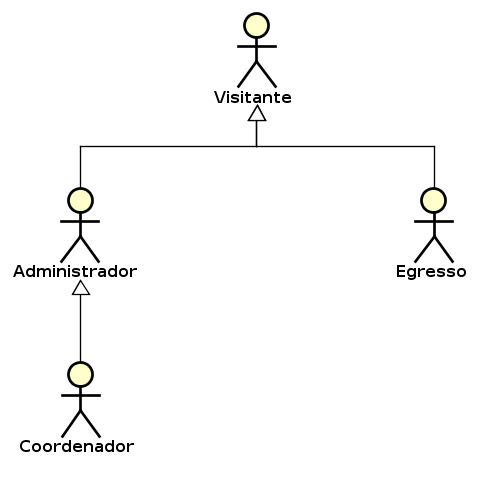
\includegraphics[width=0.5\textwidth]{figuras/atoresHeranca}
 	\caption{Diagrama de Herança dos Atores.}
 	\label{figura-caso-de-uso-atores}
\end{figure}


A seguir, são apresentados os diagramas de casos de uso e descrições associadas, organizados por subsistema.


\newpage
\section{Subsistema Core}

A Figura~\ref{figura-caso-de-uso-core} apresenta o diagrama de casos de uso do subsistema Core.

\begin{figure}[h!]
	\centering
	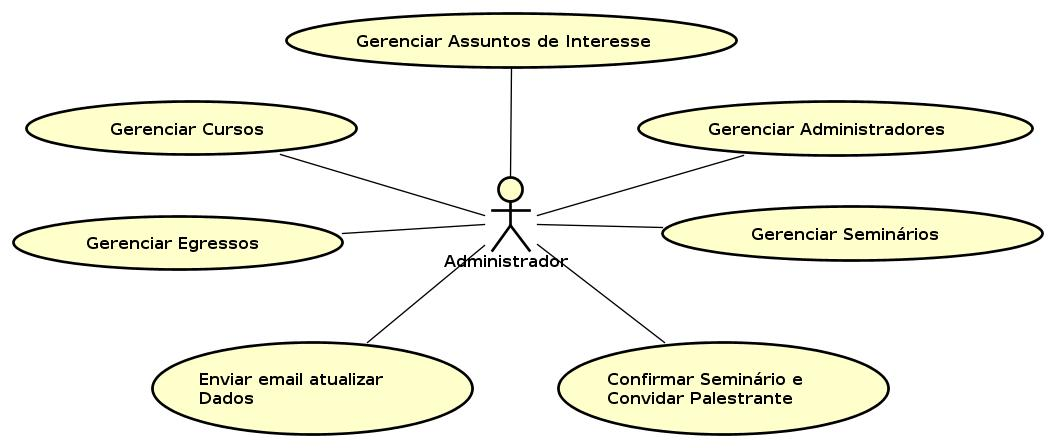
\includegraphics[width=1\textwidth]{figuras/casodeuso-core}
 	\caption{Diagrama de Casos de Uso do Subsistema Core.}
 	\label{figura-caso-de-uso-core}
\end{figure}
 
 A seguir, são apresentadas as descrições de cada um dos casos de uso identificados. Os casos de uso cadastrais de baixa complexidade, envolvendo inclusão, alteração, consulta e exclusão, são descritos na tabela~\ref{tabela-core-cadastrais}.


\newpage
\begin{table}[h]
	\centering  \vspace{0.5cm} 	\footnotesize 
	\caption{Casos de Uso Cadastrais}
	\begin{tabular}{|c|c|c|p{6cm}|c|c|} \hline  \rowcolor[rgb]{0.8,0.8,0.8}
 				
 		Id & Nome  &  Ações  &  Observações & Requisitos   & Classes  \\ 	\hline \hline	
 		
 		{}    &    {}    &   I   &    Informar: nome, email, matricula e CPF. Será criada uma senha padrão, e assim que o administrador fizer o primeiro acesso, o sistema solicitará a atualização da mesma.  &   {}   &   {}    \\\cline{3-4}
 		{}  &   Gerenciar    &   A   &   {}   &    {}   &    {}  \\ \cline{3-4}
 		\UC\label{uc-administrador}  &  Administradores  &  C  &   {}    &   RF-1  &   Administrador    \\\cline{3-4}
 	    {}   &  {}   &    E    &    Não é permitido excluir um administrador que é coordenador de um curso.   &  {}  &  {} \\ \hline \hline
 		
 		
 		
 		\rowcolor[rgb]{0.97,0.97,0.97}
 		{}   &  {}   &  I  &   Informar: nome, código e coordenador (deve ser escolhido dentre os administradores cadastrados).   &  {}   &  {}    \\ \cline{3-4} \rowcolor[rgb]{0.97,0.97,0.97}
 		{} &   Gerenciar   &   A   &   {}   &    {}  &    {}   \\ \cline{3-4} \rowcolor[rgb]{0.97,0.97,0.97}
 		\UC\label{uc-curso} &    Cursos   &  C  &  {}  &  RF-3  &  Curso \\ \cline{3-4} \rowcolor[rgb]{0.97,0.97,0.97} 
 		{}    &    {}     &   E   &    Não é permitido excluir um curso que tenha egressos associados.  &  {}   & {} \\ \hline \hline
 		  
 		  
 		  
 		          
 		{}     &   {}    &   I   &    Informar: nome.     &   {}   &    {}    \\ \cline{3-4}
 		{}  &   Gerenciar   &   A   &   {}      &   {}    &    Assunto de   \\\cline{3-4}
 		\UC\label{uc-assunto}  &    Assuntos de   &    C   &    {}     &  RF-4  &    Interesse   \\\cline{3-4}
 		{} & interesse & E & Não é permitido excluir um assunto que tenha seminários associados. & {} & {} \\ \hline \hline
 		
 		
 		
 		\rowcolor[rgb]{0.97,0.97,0.97}
 		{} & {} & {} & Informar: nome, email, CPF, data de nascimento, identidade, sexo, naturalidade e nacionalidade. & {} & {} \\ \rowcolor[rgb]{0.97,0.97,0.97} 
 		{} & Gerenciar  &  I  & O sistema ao registrar o egresso  &  RF-2  &  Egresso,   \\  \rowcolor[rgb]{0.97,0.97,0.97}
 		\UC\label{uc-egresso}  & Egressos  &  {}   &  deve enviar um email para o mesmo.  &  RF-6   &    {}     \\ \cline{3-4} \rowcolor[rgb]{0.97,0.97,0.97}
 		{}  &  {}   &  A  &   {}    &  RN-1 &    Curso Realizado   \\\cline{3-4} \rowcolor[rgb]{0.97,0.97,0.97}
 		{}  &  {}   &  C  &   {}    &   RF-7   &    {}   \\\cline{3-4} \rowcolor[rgb]{0.97,0.97,0.97}
 		{}  &  {}   &  E  &   Não é permitido excluir egressos.   &  {}   &  {}  \\ \hline \hline
 		
 		
 		
		{}  &  {}  &  I  &  Informar: titulo, palestrante, data, local e assunto de interesse.  &  {}  &  {}  \\ \cline{3-4}
 		{} & {}  &  A  &  Caso o seminário já tenha sido confirmado e enviado email, o sistema deve enviar um email aos egressos informandos as alterações. & {} & {} \\ \cline{3-4}
 		\UC\label{uc-seminario}   &  Gerenciar   &    C   &    {}     &  RF-5   &    Seminário   \\ \cline{3-4}
 		{}    &    Seminários   &  E  &  Caso o seminário já tenha sido confirmado e enviado email, o sistema deve enviar um email aos egressos informandos a exclusão do seminário.  &  {}   &  {}   \\ \hline 
 		 		
 		 		
	\end{tabular}
	\label{tabela-core-cadastrais}
\end{table}




\newpage
\begin{flushright}    \textbf{Descrição de Caso de Uso}   \end{flushright}         
\noindent  \textbf{Projeto:} \imprimirtitulo  \\ 
\textbf{Identificador do Caso de Uso:} \UC\label{uc-seminario} \\ 
\textbf{Caso de Uso:} Confirmar Seminário e Convidar Palestrante \\
\noindent \textbf{Descrição Sucinta:} Este caso de uso é responsável por confirmar a ocorrência de seminários e por convidar egressos para se apresentarem como palestrantes.\\

\begin{table}[h]
	\centering    \vspace{0.5cm}     \footnotesize
	\caption{Fluxos de Eventos Normais}
	\begin{tabular}{|p{2.3cm}|p{1.8cm}|p{10.7cm}|} \hline  \rowcolor[rgb]{0.8,0.8,0.8}
 					
 		Nome do Fluxo & Precondição & Descrição  \\ \hline		
		
		Confirmar & {} & 1. O administrador informa o seminário a ser confirmado.  \\
		Seminário & {} & 2. O sistema envia email a todos os egressos que tenham interesse naquele assunto.\\ \hline 
			
		Convidar & {} & 1. O administrador informa o seminário sem palestrante.  \\
		Palestrante & {} & 2. O sistema envia email a todos os egressos que tenham interesse naquele assunto, convidando-os a serem o palestrante.\\ \hline 
		
		
		Voluntariar & {} & 1. O egresso informa o assunto e voluntaria-se como palestrante.  \\
		Palestrante & {} & 2. O sistema envia um email para informar o administrador.\\ \hline 
		
	\end{tabular}	
\end{table}

	\begin{table}[h]
		\centering 	\vspace{0.5cm}    \footnotesize
		\caption{Fluxos de Eventos Variantes}
		\begin{tabular}{|p{4.3cm}|p{3.5cm}|p{7.0cm}|}    \hline  \rowcolor[rgb]{0.8,0.8,0.8}
 		
 			Fluxo Relacionado &  Variante  &  Descrição    \\	\hline		
		
			Voluntariar Palestrante/  & 2 - O envio de email      & 2a - O sistema envia um email para o usuário   \\ 
			Confirmar Seminário / 	  & retorna um erro.			&  que instalou o sistema informando do erro. \\
			Convidar Palestrante     &{}              & 3 - O sistema retorna uma mensagem de erro ao usuário. \\\hline
		
		\end{tabular}
	\end{table}	
	
	

\noindent  \textbf{Requisitos Relacionados:} RF-5, RF-16     \\ \textbf{Classes Relacionadas:} Seminário. 





\newpage
\begin{flushright}    \textbf{Descrição de Caso de Uso}   \end{flushright} 
\noindent \textbf{Projeto:} \imprimirtitulo \\
\textbf{Identificador do Caso de Uso:} \UC\label{uc-email-atualizar-dados}\\ 
\textbf{Caso de Uso:} Enviar email atualizar dados \\
\noindent \textbf{Descrição Sucinta:} Este caso de uso é responsável enviar para os egressos a cada 2 anos um email solicitando a atualização de seus dados.\\

\begin{table}[h]
	\centering 	\vspace{0.5cm} 	\footnotesize
	\caption{Fluxos de Eventos Normais}
	\begin{tabular}{|p{2.3cm}|p{1.1cm}|p{11.4cm}|} \hline  \rowcolor[rgb]{0.8,0.8,0.8}
 					
 		Nome do Fluxo & Precond. & Descrição  \\ \hline		
	
		Enviar email & {} & 1. O sistema verifica se o último pedido de atualização tem mais de 2 anos. \\ 
		
		{} & {} & 2. O administrador sendo alertado pelo sistema, envia email a todos o egressos. \\ \hline
		
		
				
	\end{tabular}	
\end{table}


	\begin{table}[h]
		\centering 	\vspace{0.5cm}    \footnotesize
		\caption{Fluxos de Eventos Variantes}
		\begin{tabular}{|p{3.8cm}|p{4cm}|p{7.0cm}|}    \hline  \rowcolor[rgb]{0.8,0.8,0.8}
 		
 			Fluxo Relacionado &  Variante  &  Descrição    \\	\hline		
		
			Enviar  		& 2 - O envio de email      & 2a - O sistema envia um email para o usuário   \\ 
			email		& retorna um erro.			&  que instalou o sistema informando do erro. \\
			{}    		&{}              			& 3 - O sistema retorna uma mensagem de erro ao usuário. \\\hline
		
		\end{tabular}
	\end{table}	

\noindent  \textbf{Requisitos Relacionados:} RF-12   %  \\ \textbf{Classes Relacionadas:} 












\newpage
\section{Subsistema Public}

A Figura~\ref{figura-caso-de-uso-public}  apresenta o diagrama de casos de uso do subsistema Public.

\begin{figure}[h!]
  \centering
  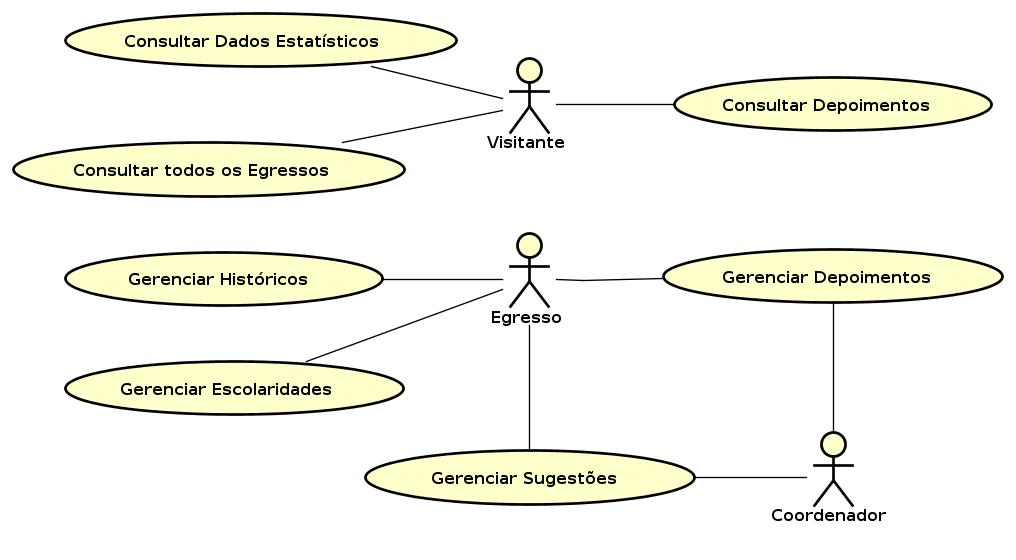
\includegraphics[width=1\textwidth]{figuras/casodeuso-public.jpg}
  \caption{Diagrama de Casos de Uso do Subsistema Public.}
  \label{figura-caso-de-uso-public}
\end{figure} 


Os casos de uso cadastrais de baixa complexidade, envolvendo inclusão, alteração, consulta e exclusão, são descritos na tabela~\ref{tabela-public-cadastrais}.

\begin{table}[h]
	\centering  \vspace{0.5cm} 	\footnotesize 
	\caption{Casos de Uso Cadastrais}
	\begin{tabular}{|c|c|c|p{6cm}|c|c|} \hline  \rowcolor[rgb]{0.8,0.8,0.8}
 				
 		Id & Nome  &  Ações  &  Observações & Requisitos   & Classes  \\ 	\hline 
 		
 		{}    &    {}    &   I   &    Informar: titulo, ano, intituição, estado e o país.  &   {}   &   {}    \\\cline{3-4}
 		\UC\label{uc-escolaridade}  &   Gerenciar    &   A  , C   &   {}   &    RF-14   &    Escolaridade  \\ \cline{3-4}
 		{}  & Escolaridades  &  E  &   {}    &   {}  &   {}  \\ \hline 
 		
 		{}    &    {}    &   I   &    Informar: faixa salarial, area de atuação, se atua na area de formação, o nível de escolaridade e se reside no Espirito Santo .  &   {}   &     \\\cline{3-4}
 		\UC\label{uc-historico}  &   Gerenciar    &   A  , C   &   {}   &    RF-14   &  Histórico      \\ \cline{3-4}
 		{}  & Histórico   &  E  &   {}    &   {}  &   do Egresso  \\ \hline 
 		
	\end{tabular}
	\label{tabela-public-cadastrais}
\end{table}




\newpage
Os casos de uso de consulta mais abrangente que as consulta a um único objeto, mas ainda de baixa complexidade, estão descritos na tabela~\ref{tabela-public-consulta}.

\begin{table}[h]
	\centering  \vspace{0.5cm} 	\footnotesize 
	\caption{Casos de Uso de Consulta}
	\begin{tabular}{|c|c|p{8cm}|c|c|} \hline  \rowcolor[rgb]{0.8,0.8,0.8}
 				
 		Id & Nome   &  Observações & Requisitos   & Classes  \\ 	\hline	
 		
 		{}  &  {}  &   As consultas aos egressos poderão ser feitas de forma  & {}   & {}    \\ 
 		{} &  Consultar   & geral onde serão mostrado todos os egressos, ou por  & {} & {} \\ 
 	    \UC\label{uc-consulta-todos-egresso}  &  Todos  & curso onde serão mostrados apenas os egressos que  & RF-13 & Egresso \\	
 	    {}  &  Egressos   &  formaram naquele curso, será exibido na tela para ao usuário o nome do egresso, o curso que realizou, o ano de inicio e o ano de termino.   & {}   & {}  \\	\hline
 	    
 	    
 	    
 	    {} &  {}  &  As consultas aos depoimentos poderão ser realizadas   & {}   & {}    \\ 
 		{} &  Consultar & de forma geral onde serão mostrados todos os  & {} & {} \\ 
 	    \UC\label{uc-consulta-depoimento} & Depoimento & depoimentos, ou por curso onde serão mostrados & RF-17 & Depoimento \\	
 	    {} & {}  & apenas depoimentos sobre o curso escolhido, será exibido na tela o conteúdo, o autor e a data de postagem. & {} & {} \\	\hline
 	    
 	     				
	\end{tabular}
	\label{tabela-public-consulta}
\end{table}




\newpage
\begin{flushright}    \textbf{Descrição de Caso de Uso}   \end{flushright}         
\noindent \textbf{Projeto:} \imprimirtitulo  \\
\textbf{Identificador do Caso de Uso:} \UC\label{uc-seminario} \\
\textbf{Caso de Uso:} Consultar dados Estatísticos \\
\noindent \textbf{Descrição Sucinta:} Este caso de uso é responsável por gerar relatórios com dados estatísticos sobre o perfil dos egressos.\\

\begin{table}[h]
	\centering \vspace{0.5cm} \footnotesize
	\caption{Fluxos de Eventos Normais}
	\begin{tabular}{|p{2.3cm}|p{1.8cm}|p{10.7cm}|} \hline  \rowcolor[rgb]{0.8,0.8,0.8}
 					
 		Nome do Fluxo & Precondição & Descrição  \\ \hline		
					
		Gerar    & {} & 1. O visitante informa o curso.  \\
		relatório    & {} & 2. O visitante informa o tipo de relatório: faixa salarial, atuação, escolaridade, entre outros (vide Documento de Especificação de Requisitos, seção 3.1).\\ 
        {} & {} & 3. O sistema gera o gráfico e mostra ao visitante.\\	\hline 
				
	\end{tabular}
\end{table}

\noindent  \textbf{Requisitos Relacionados:} RF-13       \\ \textbf{Classes Relacionadas:} Egresso, Histórico do Egresso.





\newpage
\begin{flushright}    \textbf{Descrição de Caso de Uso}   \end{flushright} 
\noindent \textbf{Projeto:} \imprimirtitulo \\
\textbf{Identificador do Caso de Uso:} \UC\label{uc-sugestao}\\ 
\textbf{Caso de Uso:} Gerenciar Sugestões \\
\noindent \textbf{Descrição Sucinta:} Este caso de uso é responsável gerenciar as sugestões enviadas pelos egressos.\\

\begin{table}[h]
	\centering 	\vspace{0.5cm} 	\footnotesize
	\caption{Fluxos de Eventos Normais}
	\begin{tabular}{|p{2.3cm}|p{1.8cm}|p{10.7cm}|} \hline  \rowcolor[rgb]{0.8,0.8,0.8}
 					
 		Nome do Fluxo & Precondição & Descrição  \\ \hline		
	
		Incluir nova  & {} & 1. O egresso informa o conteúdo da sugestão e o curso. \\ 
		Sugestão & {} & 2. O sistema preenche os campos data e autor. \\
		{} & {} & 3. O sistema envia um email ao coordenador do curso, informando da sugestão. \\ \hline
		
		Responder  & {} & 1. O coordenador seleciona a sugestão. \\ 
		Sugestão & {} & 2. O coordenador informa a resposta. \\
		{} & {} & 3. O sistema envia um email ao egresso autor da sugestão, com a resposta do coordenador. \\ \hline
				
	\end{tabular}	
\end{table}

\noindent  \textbf{Requisitos Relacionados:} RF-8, RF-11       \\ \textbf{Classes Relacionadas:} Sugestão










\newpage
\begin{flushright}    \textbf{Descrição de Caso de Uso}   \end{flushright} 
\noindent \textbf{Projeto:} \imprimirtitulo \\
\textbf{Identificador do Caso de Uso:} \UC\label{uc-depoimento}\\ 
\textbf{Caso de Uso:} Gerenciar Depoimentos \\
\noindent \textbf{Descrição Sucinta:} Este caso de uso é responsável gerenciar os depoimentos enviados pelos egressos.\\

\begin{table}[h]
	\centering 	\vspace{0.5cm} 	\footnotesize
	\caption{Fluxos de Eventos Normais}
	\begin{tabular}{|p{2.3cm}|p{1.8cm}|p{10.7cm}|} \hline  \rowcolor[rgb]{0.8,0.8,0.8}
 					
 		Nome do Fluxo & Precondição & Descrição  \\ \hline		
	
		Incluir novo & {} & 1. O egresso informa o conteúdo, se é anônimo e o curso. \\ 
		Depoimento & {} & 2. O sistema preenche os campos data e autor. \\
		{} & {} & 3. O sistema envia um email ao coordenador do curso, informando de um depoimento pendente. \\ \hline
		
		Avaliar  & {} & 1. O coordenador seleciona o depoimento pedente. \\ 
		Depoimento & {} & 2. O coordenador informa se liberado ou não liberado. \\\hline
				
		Alterar  & {} & 1. O egresso seleciona o depoimento. \\ 
		Depoimento & {} & 2. O egresso informa os novos dados. \\
		{} & {} & 3. O sistema envia um email ao coordenador do curso, informando de um depoimento pendente. \\ \hline
		
		Excluir   & {} & 1. O egresso seleciona o depoimento. \\ 
		Depoimento & {} & 2. O egresso confirma a exclusão. \\
		{} & {} & 3. O sistema exclui o depoimento. \\ \hline
				
	\end{tabular}	
\end{table}

\begin{table}[h]
	\centering 	\vspace{0.5cm}    \footnotesize
	\caption{Fluxos de Eventos Variantes}
	\begin{tabular}{|p{2.3cm}|p{4.8cm}|p{7.7cm}|}    \hline  \rowcolor[rgb]{0.8,0.8,0.8}
 		
 		Fluxo Relacionado &  Variante  &  Descrição    \\	\hline		
		
		Avaliar    & 2 - O coordenador avaliar como   & 2a - O sistema envia um email para o egresso,  \\ 
		Depoimento & não liberado & informando para refazer seu depoimento. \\\hline
		
	\end{tabular}
\end{table}

\noindent  \textbf{Requisitos Relacionados:} RF-9, RF-10     \\ \textbf{Classes Relacionadas:} Depoimento






